% pdflatex -shell-escape -interaction=nonstopmode main.tex && pdflatex -shell-escape -interaction=nonstopmode main.tex

\chapter{Definitionen}

% \begin{itemize}
%     \item Einführung in ML Algorithmen
%     \item ``Im folgenden werden wir ein paar Möglichkeiten in Betracht ziehen wie man Genetische Algorithmen für Black Box Optimierung benutzen kann''
%    \item ``Ausserdem verknüpfen wir diese mit einer Reduzierung vom Suchraum durch Fouriertransformationen und verwenden verschiedene Kodierung der Individuen, durch Normalverteilungen und direkt durch Zahlen''
% \end{itemize}

Dieses Kapitel bietet Einblick in die Grundlagen von \textbf{Genetischen Algorithmen} im Zusammenhang mit \textbf{neuronalen Netzen} und der \textbf{Cross Entropy Method}. Außerdem werden einige Verbesserungen zu den naiven Methoden besprochen, wie die Reduzierung des Suchraums durch \textbf{Fouriertransformationen} und die Einführung von einer \textbf{kooperativen Evolution} durch Hinzufügen von einer neuen Aktion zu dem Ablauf des Algorithmus.

    \section{Genetische Algorithmen}
        % ``Die Motivation von Genetischen Algorithmen kam aus der Natur bla blubb''\\
        % ``Im Folgenden behandeln wir die grundlegenden Operationen die einen GA ausmachen''

        % Ein Genetischer Algorithmus gehört zu den \textbf{unsupervised Learning} Methoden, die sich als Ziel setzen eine verborgene Struktur zu analysieren, ohne zu gekenntzeichnete Daten zu haben. John Holland

        Ein genetischer Algorithmus, im folgenden als \textbf{GA} abgekürzt, ist ein Optimierungsverfahren, der an von der natürlichen Selektion und Evolution inspiriert ist. Alternativ findet sich hier\cite{ga} ein formaler Leitfaden. Wir stellen uns anschaulicher Weise eine Gruppe Gazellen und einen Geparden vor.\\

        \begin{figure}[htbp]
            \begin{subfigure}{0.5\textwidth}
                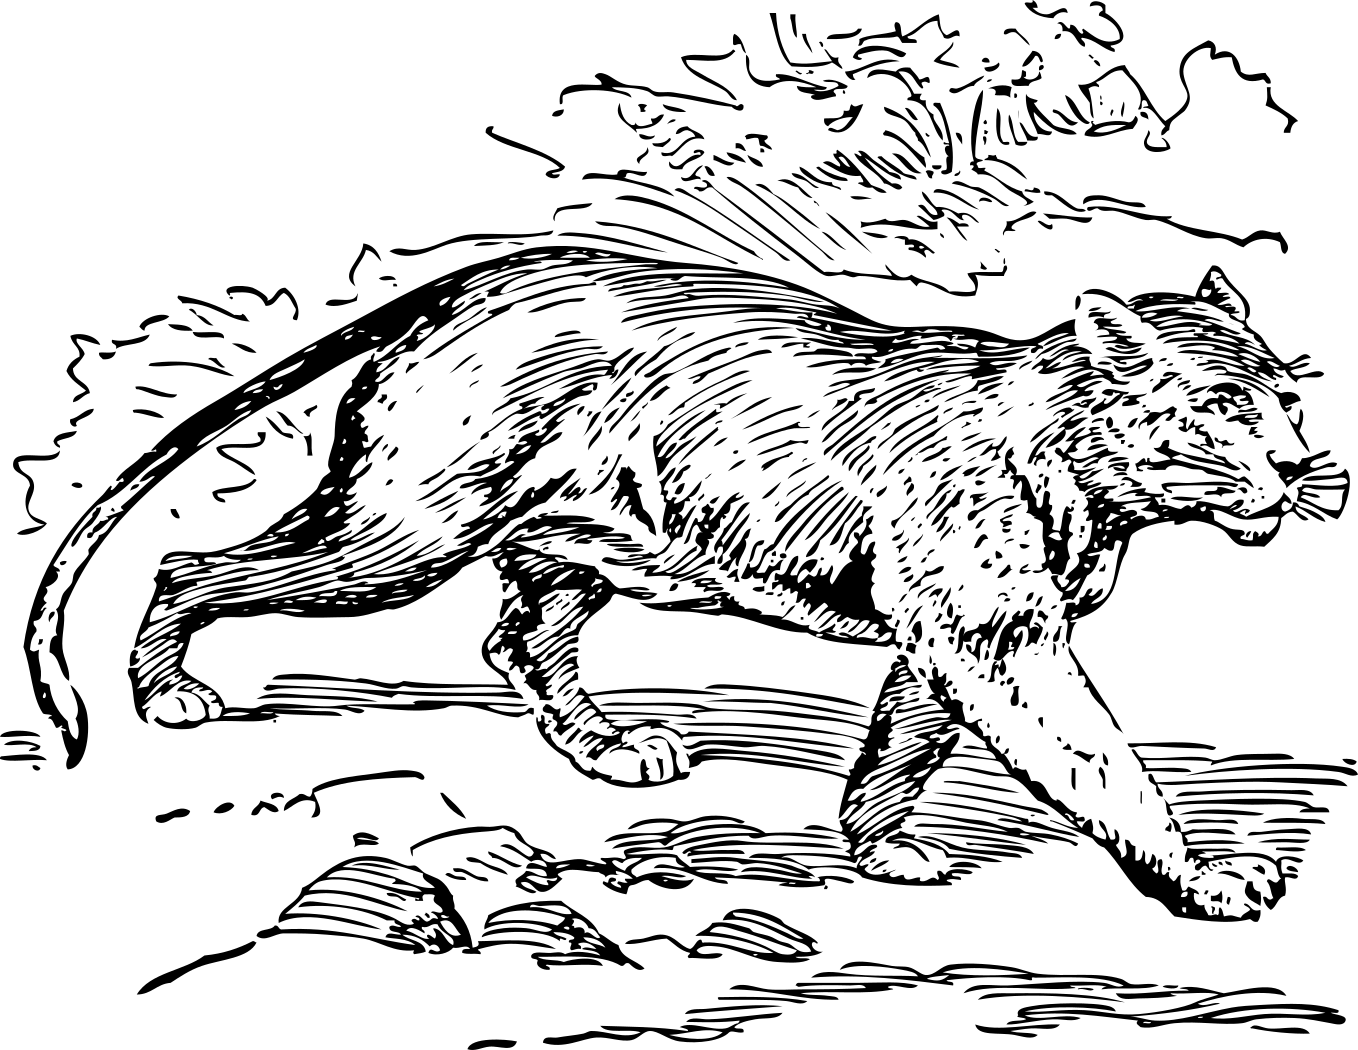
\includegraphics[width = 1\textwidth, left]{../pictures/cheetah.png}
            \end{subfigure}
            \begin{subfigure}{0.5\textwidth}
                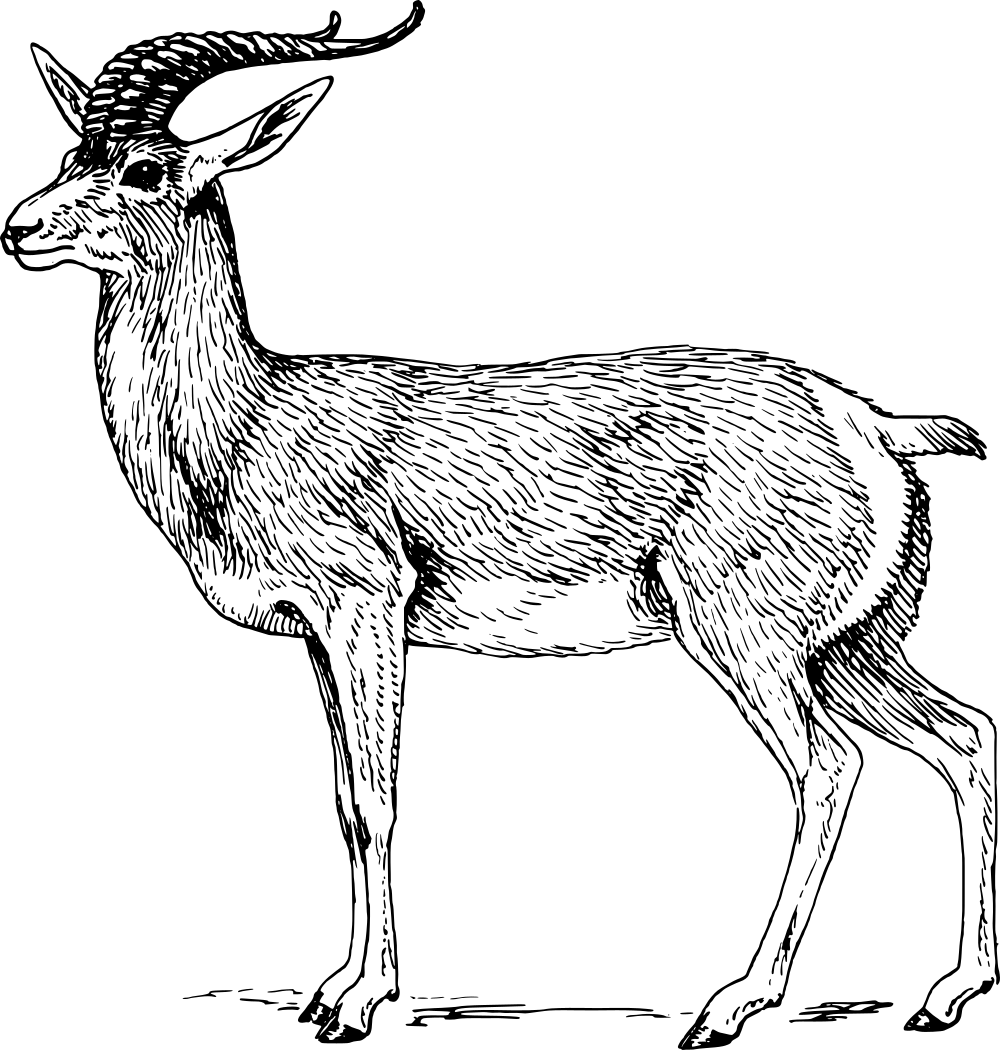
\includegraphics[width = 0.73\textwidth, right]{../pictures/gazelle.png}
            \end{subfigure}
            \caption{Illustration von einem Geparden und einer Gazelle \label{fig:gazelleAndGepard}}
        \end{figure}
        \noindent
        Sei unser Gepard durch seine Geschwindigkeit den Gazellen überlegen, dann wird die Gazellenherde über Zeit in ihrer Anzahl sinken. Dabei werden die langsamsen Gazellen dem Geparden erlegen und die Schnelleren überleben. Dieser Schritt wird als \textbf{Selektion} bezeichnet. Die Überlebenden werden sich fortpflanzen und mit hoher Wahrscheinlichkeit Gazellen-Babies bekommen die ähnlich schnell sind. Diesen Vorgang bezeichnen wir als \textbf{Kreuzung}. Mit welcher Wahrscheinlichkeit jedes einzelne Tier vor dem Geparden entwischen kann nennen wir \textbf{Fitness}.\\
        \\
        Jede Gazelle, oder auch \textbf{Individuum} genannt, hat eine eigene Fitness, die es aber bei Geburt noch nicht weiß, da sie noch nie vor einem Geparden weglaufen musste. Erst nachdem sie einmal erfolgreich entwischt ist, können wir uns vorstellen was ihre Fitness ist.\\
        \\
        Ganz selten wird ein Gazellen-Baby geboren das ein klein bisschen längere Beine hat als alle anderen, dabei hatte keiner dieses Merkmal vor ihr. Das erlaubt ihr schneller zu Laufen, was für sie erstmal positiv ist, leider hat diese Ausprägung aber den Nachteil, dass die Standhaftigkeit darunter leidet. Dieser unerwartete Veränderung in den Kindern heißt \textbf{Mutation}.\\
        \\
        Fassen wir zusammen; Nachdem jede Gazelle die nach dem Raubkatzenangriff überlebt und sich fortgepflanzt hat, bekommen wir hoffentlich wieder eine vollzähliges Herde, die wir \textbf{Population} nennen. Nach all diesen Schritten fängt der Kampf um das Überleben wieder an und geht solange, bis sich entweder Gazellen entwickeln die dem Gepard ständig entkommen können, oder bis die gesamte Population ausstirbt.\\
        \\
        Damit haben wir die wichtigsten Begrifflichkeiten von einem genetischen Algorithmus erklärt und kommen zu der Frage wie wir ihn umsetzen.

        \subsection{Individuen}

            Ein Individuum besteht aus einer Kodierung, auch \textbf{Zustandsraum} genannt, die die aussagekräftigen Eigenschaften von ihm ausmachen. Für eine Gazelle wäre beispielweise die folgende Kodierung möglich.

            \begin{multicols}{2}
                \hfill \\[-10mm]
                \begin{table}[H]
                    \begin{center}
                    \begin{tabular}{ |l|r| } 
                        \hline
                        Höchstgeschwindigkeit    & $ 95\; \frac{km}{h}$   \\ \hline
                        Beinlänge                & $ 86\; cm          $   \\ \hline
                        Gewicht                  & $ 43\; kg          $   \\ \hline
                        Hornlänge                & $ 12\; cm          $   \\ \hline
                    \end{tabular}
                    \end{center}
                    \caption{Kodierung einer Antelope \label{fig:somelabel}}
                \end{table}

                \noindent
                Die Aufgabe von unserem GA ist ein oder mehrere Individuen zu finden die es schaffen vor dem Geparden wegzulaufen. Da wir aber nicht wissen ob die vorgeschlagene Kodierung gut oder schlecht ist, müssen wir Gazellen mit zufälligen Ausprägungen erstellen und dann den Algorithmus arbeiten lassen.
            \end{multicols}
            \noindent
            Das schaffen wir indem wir Grenzen für die Kodierung festlegen und später zufällige Werte in diesen Rahmen ausprobieren.

            \begin{table}[H]
                \begin{center}
                \begin{tabular}{ |l|r|r| } 
                    \hline
                    Ausprägung               & Minimaler Wert        & Maximaler Wert       \\ \hline
                    Höchstgeschwindigkeit    & $ 20\; \frac{km}{h}$  & $ 100\; \frac{km}{h}$ \\ \hline
                    Beinlänge                & $ 40\; cm          $  & $ 90\; cm          $ \\ \hline
                    Gewicht                  & $ 12\; kg          $  & $ 75\; kg          $ \\ \hline
                    Hornlänge                & $  0\; cm          $  & $ 35\; cm          $ \\ \hline
                \end{tabular}
                \end{center}
                \caption{Grenzen für die Kodierung \cite{wiki:gazelle} \cite{blog:gazelle}\label{fig:somelabel}}
            \end{table}
            \noindent
            % Für die Kodierung unseres Individuums eignet sich ein Array von Zahlen. Um die gesamte Population darzustellen würde ein 2-dimensionales Array reichen, wobei jedes Element ein einzelnes Individuum darstellt. \textit{(evtl Grafik)}

        \subsection{Simulation}
            Nachdem wir unsere Population an Gazellen erstellt haben, müssen wir sie in eine Simulationsumgebung schicken, die ihre Fitness misst. In unserem Beispiel müssten wir eine Physiksimulation mit einem Geparden programmieren, die uns nach einer Zeitspanne sagt welche Gazellen überlebt haben. Man muss beachten dass die Komplexität der Simulation einen großen Einfluss darauf hat ob der GA eine Lösung finden kann. $ $\textit{(Grafik)}


        \subsection{Selektion}
            % ``Die besten x prozent werden genommen''

            Nachdem die Simulation vorbei ist, bekommen wir eine Population von Antilopen die jeweils überlebt hat oder nicht. Da die Fitness ist in diesem Fall binär ist, sortieren wir die Herde aller Antilopen absteigend, wobei das Überleben natürlich mehr wert ist.\\
            \\
            Nach dem Sortieren müssen wir ein prozentualen Betrag wählen, wieviele Eltern wir aus der Population wählen. In unserer Implementierung nennen wir diesen Parameter $\alpha$. \textit{(Grafik)}

        \subsection{Kreuzung}
            
            Die guten Individuen wurden ausgewählt und können sich fortpflanzen. Dafür nehmen wir jeweils zwei Individuen und nehmen zufällig die Ausprägungen von jeweils dem Vater und der Mutter. 
            \\[10mm]
            \begin{multicols}{2}
                \begin{table}[H]
                    \begin{center}
                    \begin{tabular}{ |r| } 
                        \hline
                        \hfill Ausprägungen  \\ \hline
                        \cellcolor{blue!25} $ 56\; \frac{km}{h}$ \\ \hline
                        \cellcolor{blue!25} $ 42\; cm          $ \\ \hline
                        \cellcolor{blue!25} $ 51\; kg          $ \\ \hline
                        \cellcolor{blue!25} $ 10\; cm          $ \\ \hline
                    \end{tabular}
                    \end{center}
                    \caption{Kodierung des Vaters \label{fig:somelabel}}
                \end{table}

                \begin{table}[H]
                    \begin{center}
                    \begin{tabular}{ |r| } 
                        \hline
                        \hfill Ausprägungen  \\ \hline
                        \cellcolor{yellow!25} $ 62\; \frac{km}{h}$ \\ \hline
                        \cellcolor{yellow!25} $ 55\; cm          $ \\ \hline
                        \cellcolor{yellow!25} $ 49\; kg          $ \\ \hline
                        \cellcolor{yellow!25} $  8\; cm          $ \\ \hline
                    \end{tabular}
                    \end{center}
                    \caption{Kodierung der Mutter \label{fig:somelabel}}
                \end{table}

            \end{multicols}

            \begin{multicols}{2}
                \begin{table}[H]
                    \begin{center}
                    \begin{tabular}{ |r| } 
                        \hline
                        \hfill Ausprägungen  \\ \hline
                        \cellcolor{blue!25}   $ 56\; \frac{km}{h}$ \\ \hline
                        \cellcolor{yellow!25} $ 55\; cm          $ \\ \hline
                        \cellcolor{yellow!25} $ 49\; kg          $ \\ \hline
                        \cellcolor{blue!25}   $ 10\; cm          $ \\ \hline
                    \end{tabular}
                    \end{center}
                    \caption{Kodierung vom Kind Nr.1 \label{fig:somelabel}}
                \end{table}


                \begin{table}[H]
                    \begin{center}
                    \begin{tabular}{ |r| } 
                        \hline
                        \hfill Ausprägungen  \\ \hline
                        \cellcolor{yellow!25} $ 62\; \frac{km}{h}$ \\ \hline
                        \cellcolor{blue!25}   $ 42\; cm          $ \\ \hline
                        \cellcolor{blue!25}   $ 51\; kg          $ \\ \hline
                        \cellcolor{yellow!25} $  8\; cm          $ \\ \hline
                    \end{tabular}
                    \end{center}
                    \caption{Kodierung vom Kind Nr.2 \label{fig:somelabel}}
                \end{table}
            \end{multicols}

            In unserem Beispiel haben wir die Kinder mit dem folgenden Python Code konstruiert.
            \begin{minted}[escapeinside=||, xleftmargin=-50pt]{python}
                vater  = [56,42,51,10]
                mutter = [62,55,49,8]
                kind1  = []
                kind2  = []
                for i in range(kodierung.length):
                    r = random.uniform(0,1)
                    if (r > 0.5):
                        kind1[i] = vater[i]
                        kind2[i] = mutter[i]
                    else:
                        kind1[i] = mutter[i]
                        kind2[i] = vater[i]
            \end{minted}
            \noindent
            Diese Art und Weise zwei Individuen zu kreuzen nennt sich \textbf{n-point crossover}, weil wir die Kodierung an undefiniert vielen Stellen unterbrechen und wieder zusammensetzen. Es gibt noch andere Kreuzungsmethoden die eine eine feste Anzahl von Aufteilungen benutzen, wie \textbf{one-} oder \textbf{two-point crossover}. \\
            \\
            \noindent
            Um einen Unterschied zwischen diesen Methoden zu erkennen, stellen wir uns vor dass das Alter in Zusammenhang mit der Höchstgeschwindigkeit steht, weil ältere Tiere nicht mehr die Leistung bringen können die sie mal gebracht haben. Wenn nun ein Kind gezeugt wird, dass in unserem Beispiel ein hohes Alter vererbt, bringt ihm die Höchstgeschwindikeit nichts mehr. Deshalb wäre es besser, wenn diese Ausprägungen zusammen übernommen werden, weil dadurch eine höhere Fitness garantiert werden kann. Kreuzungsmethoden die die Kodierung nicht oft aufspalten verletzen diese Eigenschaft seltener als \textit{n-point crossover}.\\
            \\
            \noindent
            Es ist zu beachten dass je nach Implementierung nur eins der beiden Kinder weiter verwendet wird, weil dann die Repopulation einfach  einfacher ist, die Varianz nicht zu stark gesenkt wird und keinerlei Information verloren geht, weil die Eltern in der Population die Kodierung weiter tragen.


        \subsection{Mutation}
%            ``Mutation ist hilfreich um die Varianz der Population etwas zu erhöhen'' \\
            Nachdem die Kinder erstellt wurden, müssen wir die Kodierung der Individuen etwas verändern, damit die Varianz in der Gesamtpopulation erhöht wird. Das machen wir indem wir durch die Kodierung der Kinder durchgehen und jede Ausprägung mit einer geringen Wahrscheinlichkeit verändern. Diese nennen wir $\beta$.

            \begin{multicols}{2}
                \begin{table}[H]
                    \begin{center}
                    \begin{tabular}{ |r| } 
                        \hline
                        \hfill Ausprägungen  \\ \hline
                        \cellcolor{yellow!25} $ 62\; \frac{km}{h}$ \\ \hline
                        \cellcolor{blue!25}   $ 42\; cm          $ \\ \hline
                        \cellcolor{blue!25}   $ 51\; kg          $ \\ \hline
                        \cellcolor{yellow!25} $  8               $ \\ \hline
                    \end{tabular}
                    \end{center}
                    \caption{Kodierung vom Kind Nr.2 \label{fig:somelabel}}
                \end{table}

                \begin{table}[H]
                    \begin{center}
                    \begin{tabular}{ |r| } 
                        \hline
                        \hfill Ausprägungen  \\ \hline
                        \cellcolor{yellow!25} $ 62\; \frac{km}{h}$ \\ \hline
                        \cellcolor{blue!25}   $ 42\; cm          $ \\ \hline
                        \cellcolor{red!25}    $ 45\; kg          $ \\ \hline
                        \cellcolor{yellow!25} $  8               $ \\ \hline
                    \end{tabular}
                    \end{center}
                    \caption{Mutierte Kodierung vom Kind Nr.2 \label{fig:somelabel}}
                \end{table}
            \end{multicols}
\newpage
            Der Python Code sieht hier folgendermaßen aus:
            \begin{minted}[escapeinside=||, xleftmargin=-50pt]{python}
                kinder = [k1, k2...]
                beta   = 0.1
                for i in range(kinder.length):
                    for j in range(kodierung.length):
                        if (r > beta):
                            kinder[i][j] = sampleNewFrom(kodierung[j].range)
            \end{minted}
            \noindent
            Dieser Schritt ist wichtig damit man die Möglichkeit hat aus lokalen Fitnessminimas rauszukommen, weil es schnell passieren kann dass sich über Generationen gleichwertige Ausprägungen weiterverbreiten, da sie die derzeit beste Lösung vorschlagen. Ohne Mutation würde der GA zu dieser Lösung konvergieren ohne Bessere in Betracht zu ziehen.\\
            \\
            \noindent
            In manchen Fällen kann man die Mutation noch weiter parametrisieren indem man ein Veränderungsfaktor als Argument hinzufügt. Diese Technik benutzt man, wenn die Kodierung nicht trivialerweise verändert werden kann, da sonst bestimmte Eigenschaften verloren gehen. In Kapitel 3 wird genau so ein Fall besprochen, weil wir unsere Individuen durch eine Wahrscheinlichkeitsverteilung darstellen. 

        \subsection{Repopulation}
            % ``Ist ein Schritt der oft implizit beim Crossover passiert, (zitat finden), wird nicht nur benutzt um Kinder und Eltern zu verknüpfen, sondern auch völlig neue Individuen hinzuzufügen''

            Die Eltern wurden ausgewählt, die Kindern gezeugt und mutiert, nun müssen wir die Population in eine Form bringen sodass die Simulation neu gestartet werden kann. Wir stellen das Problem wieder an einem Beispiel dar.

            \begin{minted}[escapeinside=||, xleftmargin=-50pt]{python}

                population = [i1,i2,...]                  # population.length = 10
                alpha      = 0.4
                eltern     = selection(population, alpha) # eltern.length = 4
                kinder     = crossover(eltern)            # kinder.length = 4
                beta       = 0.1
                mutkinder  = mutation(kinder, beta)       # mutkinder.length = 4

                newpopulation = eltern + mutkinder        # newpopulation.length = 8
            \end{minted}
            \noindent
            Man kann einfach erkennen dass uns zwei Individuen zum Neustart der Simulation fehlen. Dieses Problem kann man auf viele Weisen angehen, die ihre Vorteile und Nachteile haben. 

            \subsubsection*{Mehr Kinder erstellen}
                Es ist möglich während der Kreuzung solange Kinder zu erzeugen, bis die Population wieder ihre Ausgangsgröße angenommen hat. Ein Vorteil wäre, dass diese Individuen mit wahrscheinlich besseren Ausgangskodierungen starten als inherent Neue. Der Nachteil ist jedoch die gesenkte Varianz in der Population und die erhöhte Wahrscheinlichkeit zum Feststecken in einem loken Fitnessminima.

            \subsubsection*{Nicht selektiere Individuen nachfüllen}
                Man kann die nicht benutzen Individuen aus der vorherigen Population zum Auffüllen benutzen, was sich aber nur dadurch begründen würde, wenn die Chance besteht dass sie in der erneuten Simulation besser abschneiden als bisher. Ansonsten nehmen sie einen Platz einem potenziell besseren Individuum weg.

            \subsubsection*{Neue Individuen erstellen}
                In der unserer Implementierung haben wir uns für das Nachfüllen von inherent neuen Individuen entschieden, da dadurch die Varianz der Population angehoben wird und dadurch mehr Lösungen möglich sind. Ein Nachteil sind die Kinder die dadurch keinen Platz bekommen, aber da dadurch keine Information verloren geht ist es zu vernachlässigen.


    \section{Neuroevolution}
        ``Neuroevolution beschäftigt sich mit der Verknüpfung von Genetischen Algorithmen und Neuronalen Netzn''
        \subsection{Neuronale Netze}
                ``Neuronale Netze sind eine riesige Gleichung''\\
                ``Formel von Machine Learning zeigen'' \\
                ``Backpropagation wird angesprochen aber nicht ausführlich erklärt''\\
            \subsubsection*{Dense Ebene}
                ``Kleines Beispielnetz aufmalen und evtl durchrechnen''
            \subsubsection*{LSTM Ebene}
                ``Kleines Beispielnetz aufmalen und evtl durchrechnen''
            \subsubsection*{Softmax Ebene}
                ``Erklärung bieten wieso es sowas gibt und was für eine Formel angewendet wird''
        \subsection{Verbindung mit genetischen Algorithmen}
            ``Die Verknüpfung findet in der Kodierung von den Individuen statt - wir nehmen eine (naive) Darstellung von allen Gewichten''
            ``Problematik -> Folgerung zu DCT''

    \section{Diskrete Cosinus Transformation - DCT}
        ``Der Suchraum kann durch die sog. DCT auf beliebige Dimensionalität eingeschränkt werden, wenn bestimmte Annahmen getroffen werden können'' \\
        ``Fouriertransformationen machen folgendes...'' \\
        ``Es gibt eine Inverse die aus einem n-stelligen liste eine m-stellige macht, wo die Zahlen korelliert sind (Beispiele)''
        \subsection{Kodierung des Suchraums}
            ``Die Kodierung besteht aus eine 20-stellingen Liste wie im Paper (Cosyne), wo damit 2k Gewichte entwickelt wurden''

    \section{Cooperative Synapsen Neuroevolution - CoSyNE}
        ``CoSyNE wurde vom Prof.Dr.Schmidhuber an der ETH Zürich entwickelt und hat damit sehr viele anderen Algorithmen in den Schatten gestellt''\\
        ``Methodik, ist wie GA bloß mit einer Aktion mehr die statt spielbare `Policies', nur im Koeffizientraum entwickle'' \\
        ``Dies erlaubt eine (zitat) Kooperative Entwicklung von Koeffizienten für die nachfolgenden Inv.DCT'' \\
        ``Kein Crossover, geringe Mutation'' \\
        ``Beispiele vom Erfolg'' \\
        \subsection{Permutation}
            ``Wir transponieren, shuffeln und transponieren zurück''

    \section{Cross Entropy}
        ``Cross Entropy ist eine andere Möglichkeit um die Individuen darzustellen, anstatt von Zahlen, hab ich nun pro Coeffizient eine Normalverteilung habe mit Mean und STD'' \\
        (cite boer07)
        \subsection{Normalverteilung}
            ``Was ist eine Normalverteilung'' \\
            ``Wie programmiere ich eine Normalverteilung selber, Box-Muller, Randomness, Haskellcode Beispiel'' \\
